% ChemSim-GPU conference poster. TU Berlin corporate design, landscape A0.
% Build with XeLaTeX. Fonts: Muli (under ./fonts). Logo: real TU mark (tu-logo.pdf).
\documentclass[a0paper, landscape, 25pt]{tikzposter}

\usepackage{fontspec}
\setmainfont{Mulish}[Path=./fonts/, Extension=.ttf, UprightFont=*-Regular, BoldFont=*-Bold]
\setsansfont{Mulish}[Path=./fonts/, Extension=.ttf, UprightFont=*-Regular, BoldFont=*-Bold]
\newfontfamily\semibold{Mulish}[Path=./fonts/, Extension=.ttf, UprightFont=*-SemiBold]
\newfontfamily\extrabold{Mulish}[Path=./fonts/, Extension=.ttf, UprightFont=*-ExtraBold]
\setmonofont{Menlo}
\renewcommand{\familydefault}{\sfdefault}

\usepackage{graphicx}
\usepackage{tabularx}
\usepackage{qrcode}
\usepackage{ragged2e}
\usepackage[none]{hyphenat}
\usepackage{fontawesome5}
\usetikzlibrary{positioning, arrows.meta, calc}

% Benchmark hardware the numbers were measured on.
\newcommand{\gpuname}{NVIDIA RTX 3080 Ti (12\,GB), CUDA 13}

\tikzposterlatexaffectionproofoff

\definecolor{TUred}{HTML}{C40D1E}
\definecolor{TUdark}{HTML}{222222}
\definecolor{TUgrey}{HTML}{6E6E6E}
\definecolor{TUline}{HTML}{D2D2D2}

\newcommand{\titlefont}{\extrabold\fontsize{100}{108}\selectfont}
\newcommand{\subfont}{\semibold\fontsize{34}{42}\selectfont}
\newcommand{\headfont}{\bfseries\fontsize{38}{46}\selectfont}
\newcommand{\bodyfont}{\semibold\fontsize{25}{34}\selectfont}
\newcommand{\capfont}{\fontsize{20}{26}\selectfont}
\newcommand{\reffont}{\fontsize{18}{24}\selectfont}

\definebackgroundstyle{TUbg}{
  \draw[inner sep=0pt, line width=0pt, color=white, fill=white]
    (bottomleft) rectangle (topright);
}
\usebackgroundstyle{TUbg}

\defineblockstyle{plain}{
  titlewidthscale=1, bodywidthscale=1, titleleft,
  titleoffsetx=0pt, titleoffsety=0pt, bodyoffsetx=0pt, bodyoffsety=0pt,
  bodyverticalshift=0mm, roundedcorners=0, linewidth=0mm,
  titleinnersep=0mm, bodyinnersep=0mm
}{}
\useblockstyle{plain}
\setlength{\columnsep}{34mm}

\newcommand{\sectionhead}[1]{%
  {\headfont\textcolor{TUred}{\MakeUppercase{#1}}}\par\vspace{2mm}%
  {\color{TUred}\rule{\linewidth}{1.4mm}}\par\vspace{6mm}%
}

% ---- title band: title + logo + one straight red rule ----
\definetitlestyle{TU}{
  width=1130mm, roundedcorners=0, linewidth=0pt, innersep=0pt,
  titletotopverticalspace=26mm, titletoblockverticalspace=46mm
}{
  \coordinate (PL) at (\titleposleft, \titlepostop);
  \coordinate (PR) at (\titleposright, \titlepostop);
  \node[name=tcontent, anchor=north west, inner sep=0pt, text width=820mm] at (PL) {%
    {\titlefont\textcolor{TUdark}{ChemSim-GPU}}\\[6mm]
    {\subfont\textcolor{TUdark}{GPU-accelerated Tanimoto similarity for drug-discovery virtual screening}}\\[8mm]
    {\bodyfont\textcolor{TUdark}{Kiarash Mokhtari Dizaji}}\quad{\capfont\textcolor{TUgrey}{GPU Computing \textperiodcentered\ TU Berlin \textperiodcentered\ Summer Semester 2026}}%
  };
  \node[name=logo, anchor=north east, inner sep=0pt] at (PR) {
\includegraphics[height=46mm]{tu-logo.pdf}};
  % Rule sits below BOTH the title text and the logo, whichever hangs lower,
  % so it never cuts through the TU mark.
  \path let \p1=(tcontent.south west), \p2=(logo.south east) in
    coordinate (ry) at (0, {min(\y1,\y2)-16mm});
  \draw[TUred, line width=3mm] (PL |- ry) -- (PR |- ry);
}
\usetitlestyle{TU}
\title{}\author{}

% Narrow the column area horizontally to 1130mm so the section rules line up
% with the title bar. hmargin only -> vertical space (and bottom margin) unchanged.
\makeatletter
\geometry{hmargin=14.5mm}
\setlength{\TP@visibletextwidth}{\textwidth-2\TP@innermargin}
\makeatother

\begin{document}
\RaggedRight
\maketitle

\begin{columns}

% ================= COLUMN 1 : Problem, Why-GPU =================
\column{0.25}

\block{}{\sectionhead{Problem \& Motivation}
  \bodyfont
  Virtual screening looks through a large compound library for molecules similar
  to a known active one. Each molecule is turned into a binary fingerprint whose
  bits mark structural features.
  \vspace{16mm}

  \begin{center}
    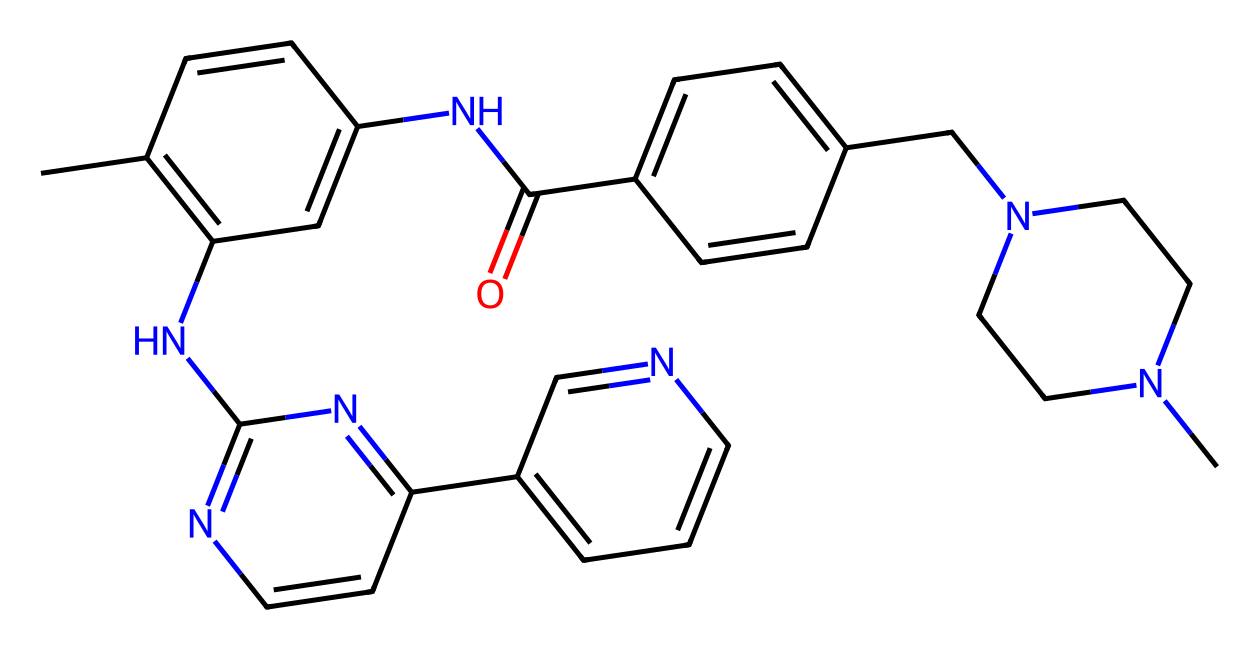
\includegraphics[width=0.90\linewidth]{mol.png}\\[5mm]
    {\capfont\textcolor{TUgrey}{Imatinib, drawn with RDKit}}\\[13mm]
    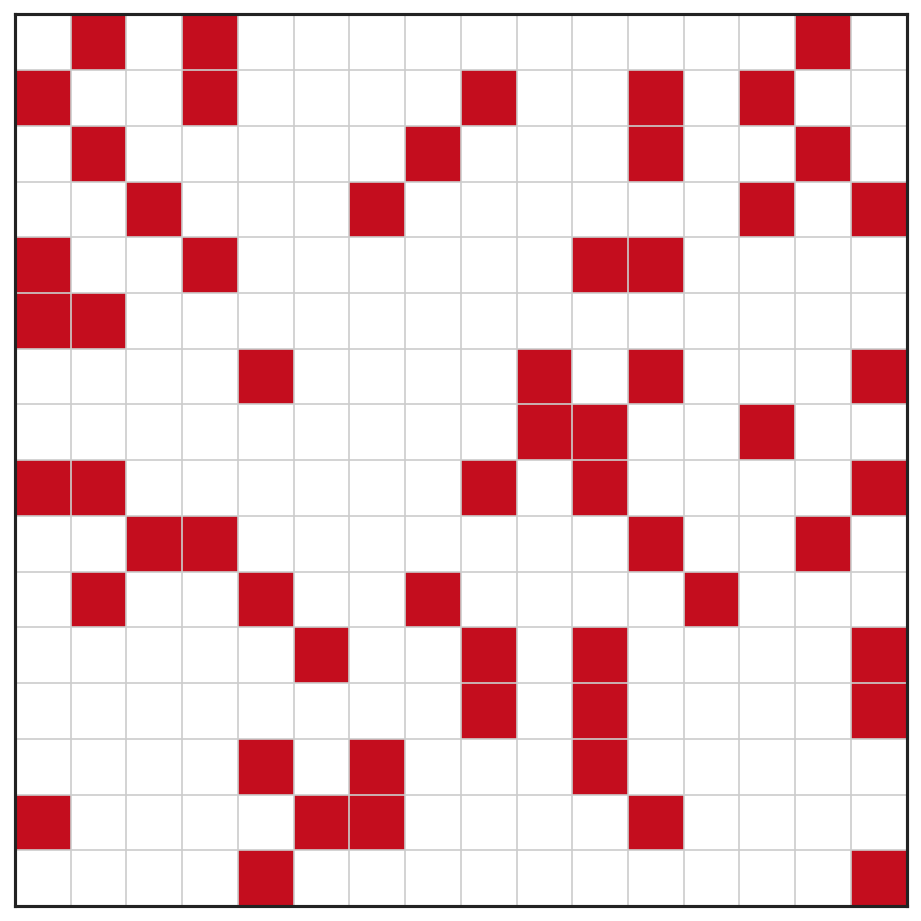
\includegraphics[width=0.64\linewidth]{fp.png}\\[5mm]
    {\capfont\textcolor{TUgrey}{Its Morgan fingerprint (shown at 256 bits; benchmarks use 1024/2048)}}
  \end{center}
  \vspace{20mm}

  Similarity is the Tanimoto coefficient:\par
  \vspace{6mm}
  {\centering\fontsize{42}{48}\selectfont\textcolor{TUdark}{$\displaystyle T=\frac{c}{a+b-c}$}\par}
  \vspace{6mm}
  where a, b, c are the popcounts of A, B, and A AND B.
  \vspace{6mm}
}

\block{}{\sectionhead{Why it fits a GPU}
  \bodyfont
  \begin{itemize}
    \setlength{\itemsep}{11mm}
    \item O(N²) output cells, all independent.
    \item No thread divergence: every thread runs the same AND plus popcount.
    \item Hardware \texttt{\_\_popcll} counts set bits in one instruction.
    \item Like a binary GEMM with popcount instead of multiply-add.
  \end{itemize}
}

% ================= COLUMN 2 : Method, Optimization Ladder =================
\column{0.25}

\block{}{\sectionhead{Method}
  \bodyfont
  \vspace{9mm}
  \centering
  \begin{tikzpicture}[node distance=17mm, every node/.style={font=\bodyfont},
      box/.style={draw=TUgrey, line width=2pt, rounded corners=3pt, fill=TUline!22,
                  text width=235mm, align=center, minimum height=36mm, inner sep=2mm},
      arr/.style={-{Stealth[length=8mm]}, TUred, line width=2.6pt}]
    \node[box] (a) {fingerprint bits};
    \node[box, below=of a] (b) {packed 64-bit words};
    \node[box, below=of b] (c) {bitwise AND + \texttt{\_\_popcll}};
    \node[box, below=of c] (e) {Tanimoto coefficient};
    \draw[arr] (a) -- (b); \draw[arr] (b) -- (c); \draw[arr] (c) -- (e);
  \end{tikzpicture}
  \vspace{26mm}
}

\block{}{\sectionhead{Optimization Ladder}
  \bodyfont
  Each stage is a separate kernel, measured against the naive baseline
  (N=8192, 2048-bit).
  \vspace{12mm}

  \begin{center}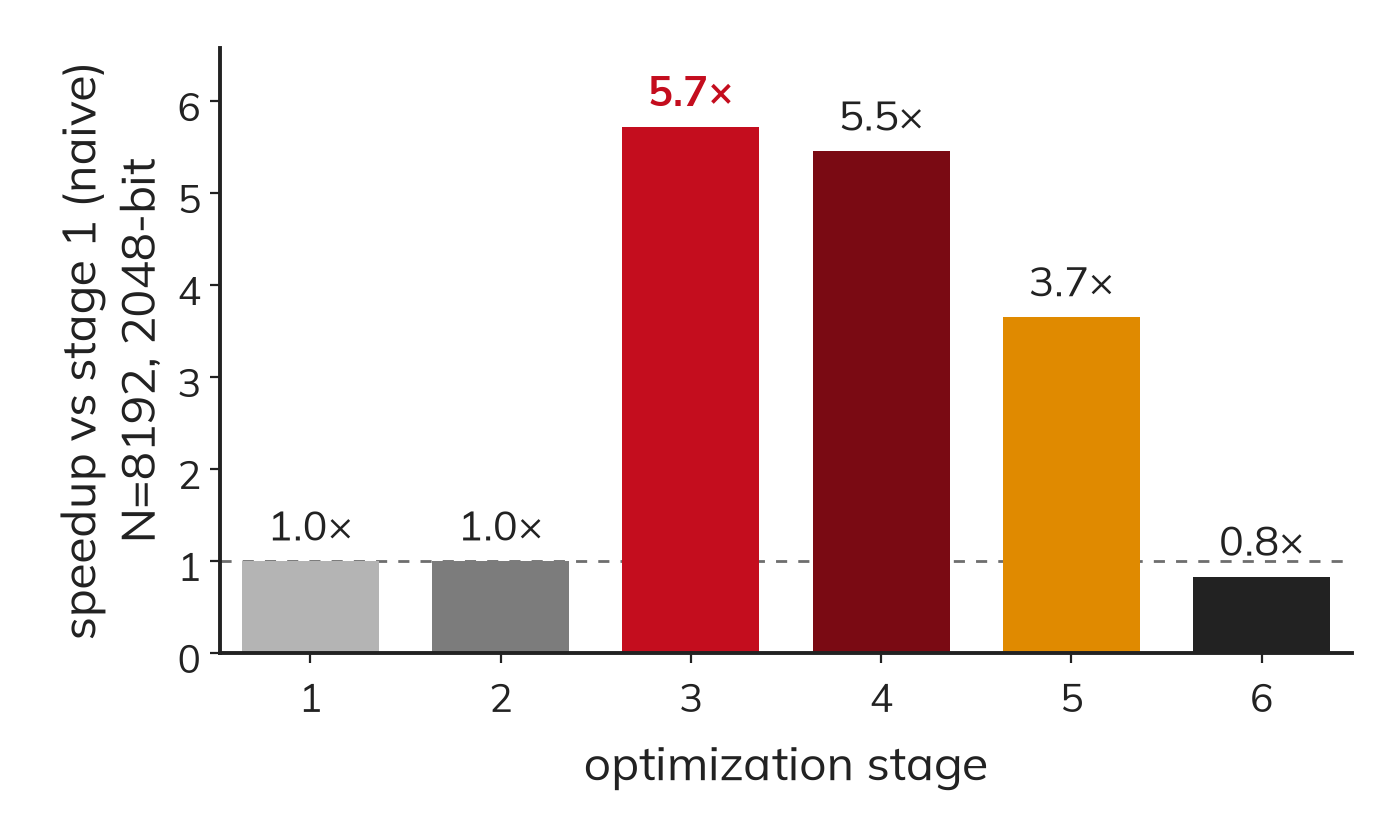
\includegraphics[width=\linewidth]{../results/speedup_ladder.png}\end{center}
  \vspace{14mm}

  \capfont
  \setlength{\tabcolsep}{2.5mm}\renewcommand{\arraystretch}{1.5}
  \begin{tabularx}{\linewidth}{@{}p{5mm} >{\raggedright\arraybackslash}p{62mm} >{\raggedright\arraybackslash}X@{}}
    \textbf{\#} & \textbf{Technique} & \textbf{What changed}\\[1mm]
    \hline\rule{0pt}{6mm}%
    1 & Naive baseline & one thread per cell, software popcount\\
    2 & Bit-pack + \texttt{\_\_popcll} & hardware popcount; still memory-bound\\
    3 & Coalescing (SoA) & adjacent threads read adjacent words\\
    4 & Shared-mem tiling & reuse fingerprints on-chip\\
    5 & Thread coarsening & reuse query word across columns\\
    6 & Warp-shuffle & lanes split words, \texttt{\_\_shfl}\\
  \end{tabularx}
  \vspace{12mm}

  {\capfont Coalescing is the big win. Coarsening and warp-shuffle regress at this
  size, the honest result that shows the memory-bound ceiling.}
}

% ================= COLUMN 3 : Correctness, Results =================
\column{0.25}

\block{}{\sectionhead{Correctness \& Validation}
  \bodyfont
  \begin{itemize}
    \item Every stage checked element-wise against a CPU reference over
      4{,}000{,}000 pairs (2000×2000); max abs error \textbf{0.0}.
    \item RDKit \texttt{BulkTanimotoSimilarity} is the reference standard.
    \item Edge cases: T(0,0)=0, identical=1, disjoint=0.
    \item Counts are exact integers, so GPU and CPU agree to float rounding.
  \end{itemize}
  \vspace{51mm}
}

\block{}{\sectionhead{Results}
  \bodyfont
  Measured on \gpuname.\par
  \vspace{6mm}
  {\centering\extrabold\fontsize{44}{50}\selectfont\textcolor{TUred}{$\sim$45 GCUPS}\par}
  \vspace{1mm}
  {\centering\capfont\textcolor{TUgrey}{peak throughput --- 1024-bit, coalesced kernel}\par}
  \vspace{9mm}

  Runtime grows as O(N²); the optimized kernel stays well below the naive one.
  \vspace{5mm}
  \begin{center}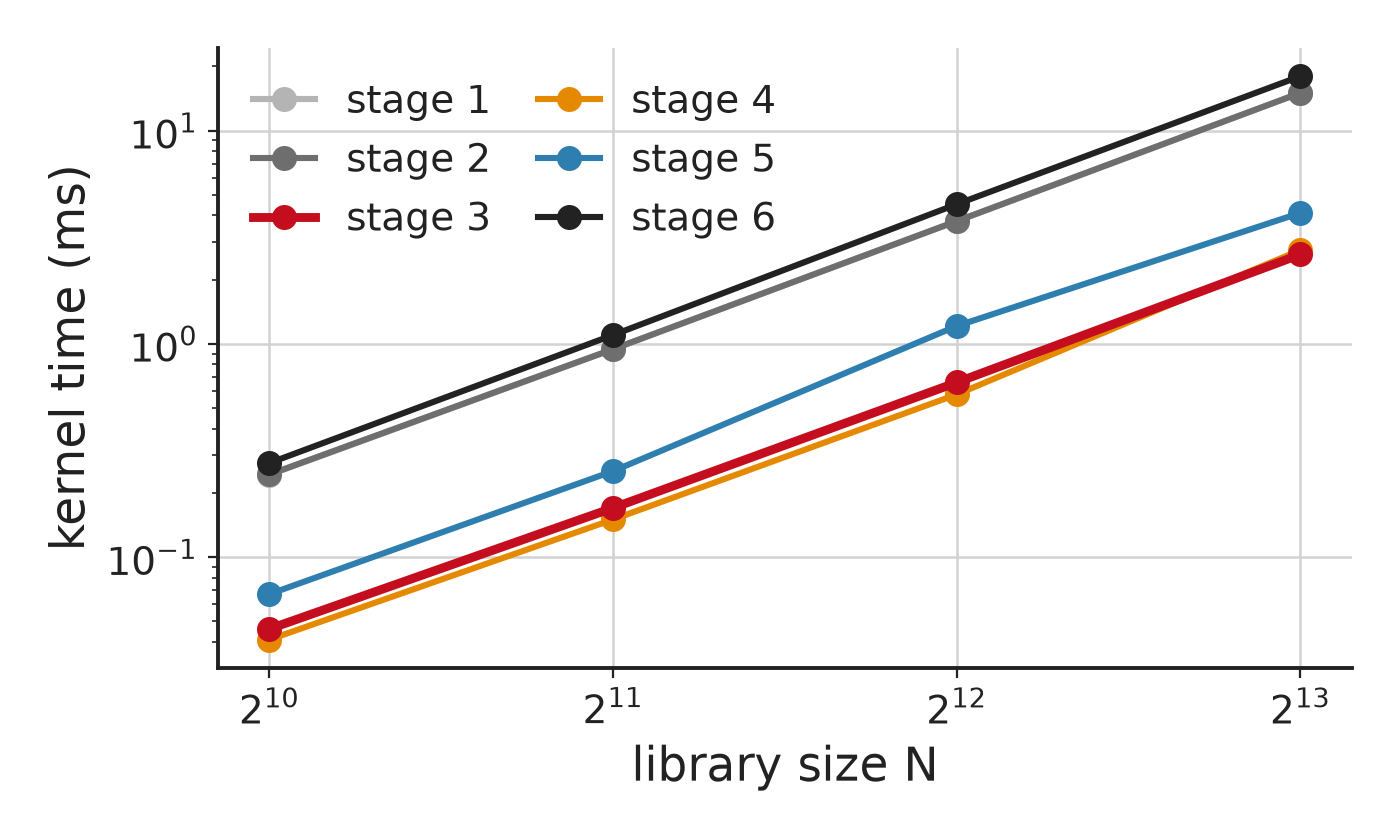
\includegraphics[width=\linewidth]{../results/scaling.png}\end{center}
  \vspace{14mm}
  Throughput peaks at coalescing, then drops as the later stages regress.
  \vspace{5mm}
  \begin{center}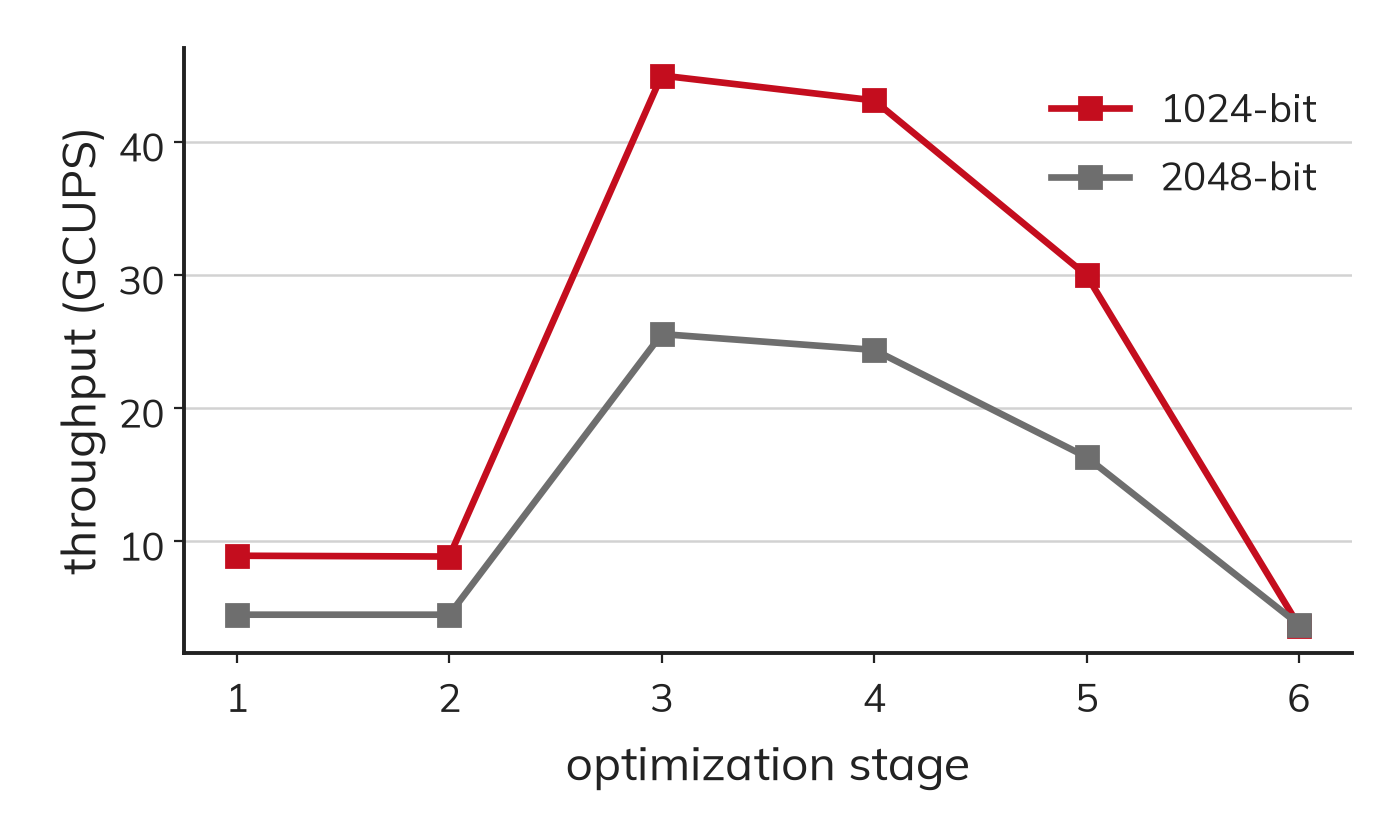
\includegraphics[width=\linewidth]{../results/gcups.png}\end{center}
}

% ================= COLUMN 4 : Conclusion, References, Code&data =================
\column{0.25}

\block{}{\sectionhead{Conclusion}
  \bodyfont
  A correct, staged CUDA engine. Coalescing gave the main gain; the kernel then
  hits a memory-bound ceiling that later stages cannot pass at this size.\par
  \vspace{7mm}
  {\centering\extrabold\fontsize{40}{46}\selectfont\textcolor{TUred}{5.7× over the naive baseline}\par}
  \vspace{14mm}

  \centering
  \begin{tikzpicture}[x=1mm, y=1mm, >={Stealth[length=6mm]}, font=\capfont]
    % memory-bound region (under the sloped roof, left of the knee)
    \fill[TUline!35] (0,0) -- (150,0) -- (150,104) -- (8,6) -- cycle;
    % axes
    \draw[TUdark, line width=1.6pt, ->] (0,0) -- (0,126);
    \draw[TUdark, line width=1.6pt, ->] (0,0) -- (232,0);
    % roofline: memory roof (slope) then compute roof (flat)
    \draw[TUred, line width=2.8pt] (8,6) -- (150,104) -- (228,104);
    % knee
    \draw[TUgrey, dashed, line width=1pt] (150,0) -- (150,104);
    % our kernel, sitting on the memory roof (white halo so it reads off the line)
    \node[circle, fill=TUdark, draw=white, line width=1.4pt,
          inner sep=0pt, minimum size=9pt] (kpt) at (104,72){};
    \draw[TUdark, line width=1pt] (kpt) -- (70,92);
    \node[anchor=east, TUdark, align=right] at (70,92) {coalesced\\kernel};
    % region + axis labels
    \node[TUgrey] at (95,20) {memory-bound};
    \node[TUgrey] at (191,46) {compute-bound};
    \node[anchor=south east, TUred] at (226,112) {compute roof};
    \node[anchor=north, TUdark] at (116,-6) {arithmetic intensity (ops / byte)};
    \node[anchor=south, rotate=90, TUdark] at (-7,63) {throughput};
  \end{tikzpicture}\par
  \vspace{4mm}
  {\capfont\textcolor{TUgrey}{The kernel sits on the memory roof: throughput
  tracks bandwidth, not compute. Coalescing uses bandwidth better and wins;
  on-chip reuse cannot lift a memory-bound kernel at this size.}\par}
  \vspace{8mm}
}

\block{}{\sectionhead{References}
  \reffont
  \begin{enumerate}
    \setlength{\itemsep}{9mm}
    \item Y. Ma, S. Wang, Y. Xie, "GPU Accelerated Chemical Similarity Calculation," J. Chem. Inf. Model., 2011.
    \item I. S. Haque, V. S. Pande, W. P. Walters, "Anatomy of High-Performance 2D Similarity Calculations," JCIM, 2011.
    \item D. Rogers, M. Hahn, "Extended-Connectivity Fingerprints," J. Chem. Inf. Model., 2010.
    \item D. Bajusz, A. R\'acz, K. H\'eberger, "Why is Tanimoto index an appropriate choice for fingerprint-based similarity calculations?," J. Cheminform., 2015.
    \item P. Willett, "Similarity-based virtual screening using 2D fingerprints," Drug Discovery Today, 2006.
    \item G. Landrum, RDKit: Open-source cheminformatics, rdkit.org.
    \item M. Harris, "Optimizing Parallel Reduction in CUDA," NVIDIA Developer Technology.
    \item NVIDIA, CUDA C++ Programming Guide (popcount intrinsics, warp-shuffle, shared memory, streams).
    \item Schr\"odinger, gpusimilarity (open-source CUDA reference).
  \end{enumerate}
  \vspace{8mm}
}

\block{}{\sectionhead{Code \& data}
  \begin{minipage}[c]{0.64\linewidth}
    \reffont\texttt{github.com/Kiarashmo/chemsim-gpu}\\[6mm]
    {\capfont\textcolor{TUgrey}{\faEnvelope[regular]\ kiarash.mokhtari.dizaji@campus.tu-berlin.de}}
  \end{minipage}\hfill
  \begin{minipage}[c]{0.32\linewidth}
    \raggedleft\qrset{height=70mm}\qrcode{https://github.com/Kiarashmo/chemsim-gpu}
  \end{minipage}
}

\end{columns}
\end{document}
